Accedendo alla \emph{Configurazione OpenVPN} (cfr. sezione \ref{rete-VPN}) nel menu, l'utente può effettuare due operazioni principali:

\begin{enumerate}[noitemsep,nolistsep]
    \item Caricare una nuova configurazione OpenVPN
    \item Visualizzare lo stato corrente della VPN
\end{enumerate}

\begin{figure}[H]
    \begin{center}
    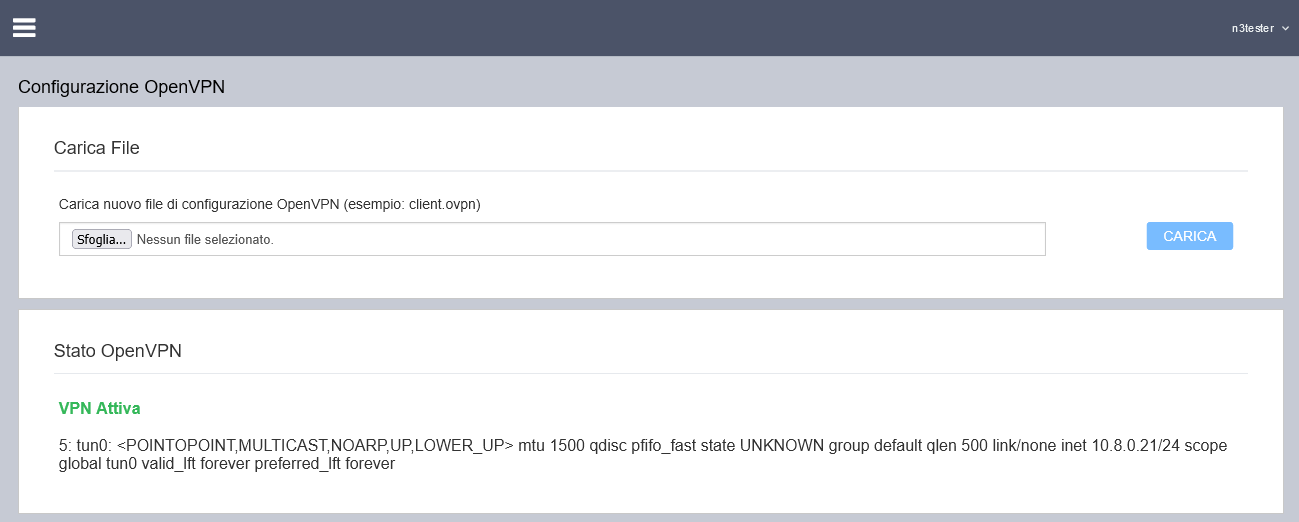
\includegraphics[width=\textwidth]{images/full-vpn.png}
    \caption{Sezione \emph{Configurazione OpenVPN}.}
    \end{center}
\end{figure}

\subsection{Caricamento nuova configurazione}

L'utente ha la possibilità di caricare un nuovo file di \textbf{configurazione OpenVPN} nell'apposita sezione, in formato \textbf{OVPN}. 

Quando il server riceve la nuova configurazione, deve prima di tutto \textbf{accedere in SSH} all'host dal container (cfr. sezione \ref{fig:containers-arch}); solo dopo essersi collegato al nodo può copiare il file di configurazione con SCP (\emph{Secure Copy}) e \textbf{riavviare la VPN}.

\begin{figure}[H]
    \begin{center}
    
\includegraphics[width=\textwidth]{images/vpn-file.png}
    \caption{Sezione per il caricamento di un nuovo file di configurazione OpenVPN.}
    \end{center}
\end{figure}

\subsection{Visualizzazione stato corrente VPN}

Oltre a poter caricare una nuova configurazione, l'utente può visualizzare lo \textbf{stato corrente} della VPN sulla macchina.

\begin{figure}[H]
    \begin{center}
    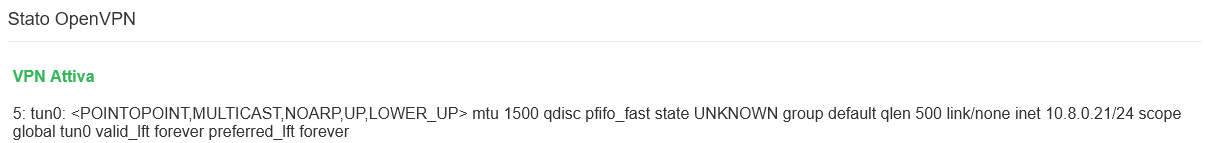
\includegraphics[width=\textwidth]{images/vpn-status.png}
    \caption{Stato corrente VPN.}
    \end{center}
\end{figure}

Per ottenere lo stato della VPN il server accede in SSH all'host e ricava le informazioni con il seguente comando eseguito nella shell:

\begin{verbatim}
    ip addr show dev tun0
\end{verbatim}